\documentclass[12pt]{article}

\usepackage[utf8]{inputenc}
\usepackage[T1]{fontenc}
%\usepackage[francais]{babel}
\usepackage{ragged2e} 

\usepackage{geometry}
\geometry{a4paper, margin=2.5cm}

\usepackage{graphicx}

\usepackage{fancybox}

\usepackage{fancyhdr}
\usepackage{lastpage}

\pagestyle{fancy}
\fancyhf{}

\rfoot{Page \thepage \hspace{1pt} of \pageref{LastPage}}

\usepackage{listings}

\usepackage{xcolor}

\definecolor{commentsColor}{rgb}{0.497495, 0.497587, 0.497464}
\definecolor{keywordsColor}{rgb}{0.000000, 0.000000, 0.635294}
\definecolor{stringColor}{rgb}{0.558215, 0.000000, 0.135316}

\lstset{
backgroundcolor = \color{white},
basicstyle = \footnotesize,
breakatwhitespace = false,
breaklines = true,
captionpos = b,
commentstyle = \color{commentsColor}\textit,
frame = tb,
keepspaces = true,
keywordstyle = \color{keywordsColor}\bfseries,
numbers = left,
numbersep = 5pt,
numberstyle = \tiny\color{commentsColor},
rulecolor = \color{black},
showspaces = false,
showstringspaces = false,
showtabs = false,
stepnumber = 1,
stringstyle = \color{stringColor},
tabsize = 2,
title = \lstname,
columns = fixed
}

\begin{document}

\newcommand{\HRule}{\rule{\linewidth}{0.125mm}}

\center
 
{ \Huge \textsc{Classification of claims\\[0.4cm] according to their veracity values}}\\[0.4cm]
\HRule \\

\justify

%\tableofcontents
%\newpage
\section{Text classification process}
Text classification is a machine learning technique that assigns a set of predefined categories to open-ended text. Text classifiers can be used to organize, structure, and categorize pretty much any text from documents or emerging social media.

In order to complete this classification task, I basically divide the data processing process into the following six:

\begin{itemize}
	\item[$\circ$] Data Acquisition
	\item[$\circ$] Text Cleaning
	\item[$\circ$] Pro-Processing
	\item[$\circ$] Feature Engineering
	\item[$\circ$] Modeling
	\item[$\circ$] Evaluation
\end{itemize}

My classification process has been shown in Figure 1.

\begin{figure}[hbtp]
	\centering \fboxrule = 0pt \fboxsep = 0pt \fcolorbox{gray}{white}{
		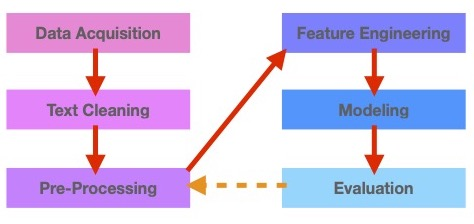
\includegraphics[width = 14cm]{figures/Figure_1.jpg}}
	\caption{Text classification process}
\end{figure}

\section{Data extraction} 

By observing the extracted data, I choose column \fbox{\textsc{claimReview\_source}} as the target column for natural language processing and column \fbox{\textsc{rating\_alternateName}} as the label for this classification learning.

However, because the values of column\fbox{\textsc{rating\_alternateName}} are not uniform, I use the python code provided by webpage GitHub to re-categorize them to generate column \fbox{\textsc{NormalizedRatings}}. And through the value of column \fbox{\textsc{NormalizedRatings}}, generate column \fbox{\textsc{label\_2c}} and column \fbox{\textsc{label\_3c}} (corresponding to two different classification methods, respectively).

\section{Tokenization}

This time,  I chose spaCy as a tool for text tokenization. The text is now pre-processed by reducing the lemmatized words (except for pronouns ('I')) and removing stop words. This process takes a long time. I only took the first data for an effect test and did not perform the operation on the entire database in the first. But this step will be completed in the process of model training.

The process of tokenization by using spaCy is as follows. (Figure 2)

\begin{figure}[hbtp]
	\centering \fboxrule = 0pt \fboxsep = 0pt \fcolorbox{gray}{white}{
		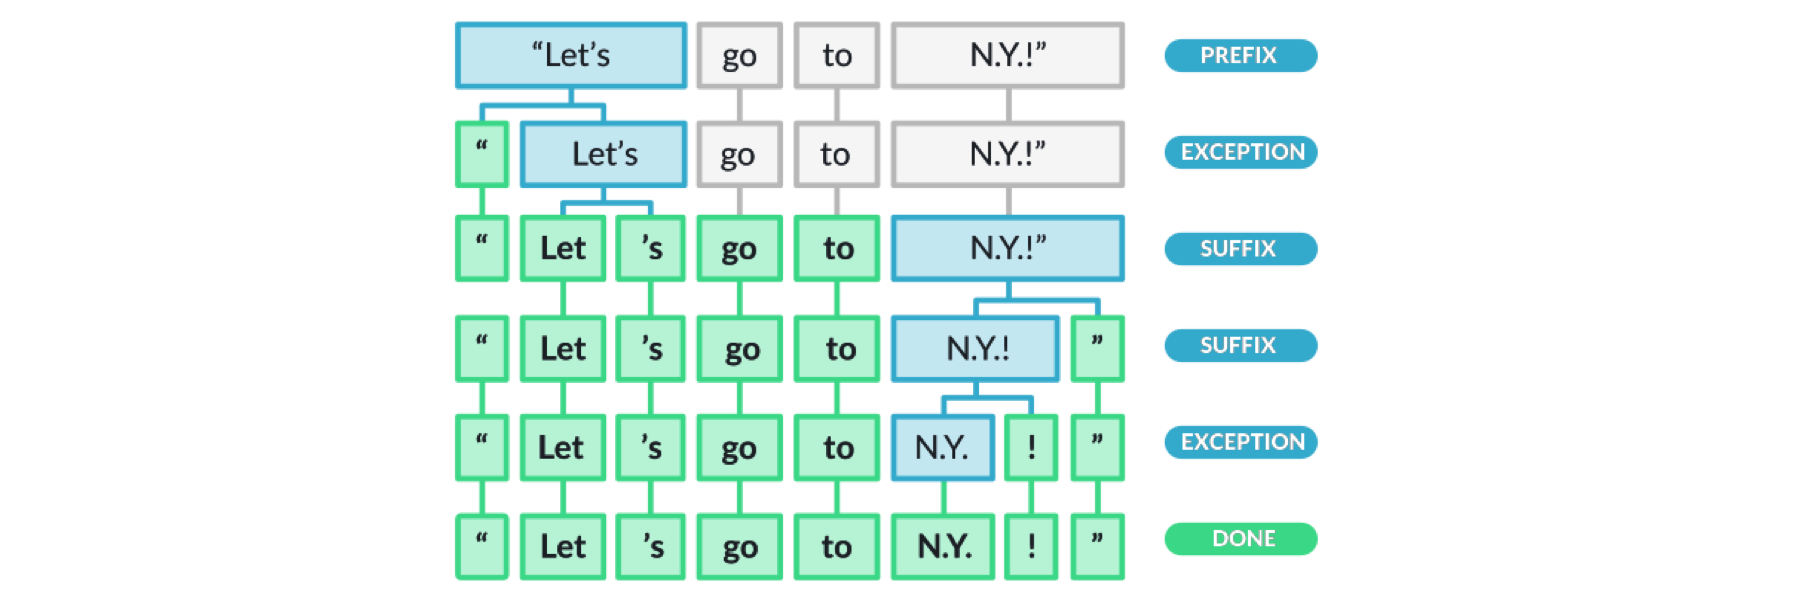
\includegraphics[width = 18cm]{figures/Figure_2.png}}
	\caption{Tokenization by spaCy}
\end{figure}

\section{Vectorization}

In the part of vectorized features, I found that some documents have the same source and a large proportion and have great potential to have the same content theme (for example, politics), so I consider adopting the TF-IDF algorithm to vectorize. In order to be able to compare, I also added the bag-of-words algorithm. After all, not all documents have the same source and have the same theme. Perhaps the bag-of-words method is more appropriate for this example.

\section{Test model}

Originally, I planned to train the model through Bayesian linear regression and support vector machine methods, and compare the exact values and confusion matrix for further analysis. It is a pity that the actual operation time is too long, and the results have not been obtained. At present, my work can only stop here. I need to recheck my code in the future to determine whether I should make improvements. Unfortunately, I couldn't get the desired result and further analysis on this in the end.

\end{document}